\setmodule{9}

%BEGIN_FOLD % ====>>_____ Занятие 1 _____<<====
\begin{class}[number=1]
	\begin{listofex}
		%11.2,3,4 по 3 первых
		\item Найдите точку максимума функции \(y=x^3-48x+17\).
		\item Найдите наименьшее значение функции \(y=x^3-27x\) на отрезке \([0;4]\).
		\item Найдите наибольшее значение функции \(y=x^3-3x+4\) на отрезке \([-2;0]\).
		\item Найдите наименьшее значение функции \(y=\dfrac{ x^2+25 }{ x }\) на отрезке \([1;10]\).
		\item Найдите точку максимума функции \(y=-\dfrac{ x^2+289 }{ x }\).
		\item Найдите точку минимума функции \(y=-\dfrac{ x^2+1 }{ x }\).
		\item Найдите наименьшее значение функции \(y=(x-8)e^{x-7}\) на отрезке \([6;8]\).
		%11.5 1-4
		\item Найдите наименьшее значение функции \(y=3x-\ln (x+3)^3\) на отрезке \([-2,5;0]\).
		\item Найдите наибольшее значение функции \(y=\ln (x+5)^5-5x\) на отрезке \([-4,5;0]\).
		\item Найдите наименьшее значение функции \(y=4x-4\ln (x+7)+3\) на отрезке \([-6,5;0]\).
		\item Найдите наибольшее значение функции \(y=8\ln (x+5)-8x+54\) на отрезке \([-6,5;0]\).
		%11-trigon 1-3
		\item Найдите наименьшее значение функции \(y=5 \cos x - 6x + 4 \) на отрезке \( \left[ -\dfrac{ 3\pi }{ 2 }; 0 \right] \).
		\item Найдите наибольшее значение функции \(y=12\cos x + 6\sqrt{3}x - 2 \sqrt{3} \pi +6 \) на отрезке \( \left[ 0; \dfrac{ \pi }{ 2 } \right] \).
		\item Найдите наименьшее значение функции \(y=3+\dfrac{ 5\pi }{ 4 } -5x - 5\sqrt{2} \cos x \) на отрезке \( \left[ 0; \dfrac{ \pi }{ 2 } \right] \).
		
		\item Изюм получается в процессе сушки винограда. Сколько килограммов винограда потребуется для получения \(20\) килограммов изюма, если виноград содержит \(90\%\) воды, а изюм содержит \(5\%\) воды?
		
		%\item Изюм получается в процессе сушки винограда. Сколько килограммов винограда потребуется для получения \(16\) килограммов изюма, если виноград содержит \(90\%\) воды, а изюм содержит \(5\%\) воды?
		%BANK https://math-ege.sdamgia.ru/test?likes=99575 // https://math-ege.sdamgia.ru/test?likes=99576 // https://math-ege.sdamgia.ru/test?likes=99576 // https://math-ege.sdamgia.ru/test?likes=99578
		%по 2
		\item Имеется два сплава. Первый сплав содержит \(5\%\) меди, второй --- \(12\%\) меди. Масса второго сплава больше массы первого на \(9\) кг. Из этих двух сплавов получили третий сплав, содержащий \(10\%\) меди. Найдите массу третьего сплава. Ответ дайте в килограммах.
		%\item Имеется два сплава. Первый сплав содержит \(5\%\) меди, второй --- \(13\%\) меди. Масса второго сплава больше массы первого на \(9\) кг. Из этих двух сплавов получили третий сплав, содержащий \(10\%\) меди. Найдите массу третьего сплава. Ответ дайте в килограммах.
		
		\item Смешав \(11\)-процентный и \(72\)-процентный растворы кислоты и добавив \(10\) кг чистой воды, получили \(31\)-процентный раствор кислоты. Если бы вместо \(10\) кг воды добавили \(10\) кг \(50\)-процентного раствора той же кислоты, то получили бы \(51\)-процентный раствор кислоты. Сколько килограммов \(11\)-процентного раствора использовали для получения смеси?
		
		
		%\item Имеется два сплава. Первый содержит \(10\%\) никеля, второй --- \(35\%\) никеля. Из этих двух сплавов получили третий сплав массой \(150\) кг, содержащий \(30\%\) никеля. На сколько килограммов масса первого сплава была меньше массы второго?
		\item Имеется два сплава. Первый содержит \(15\%\) никеля, второй --- \(35\%\) никеля. Из этих двух сплавов получили третий сплав массой \(140\) кг, содержащий \(30\%\) никеля. На сколько килограммов масса первого сплава была меньше массы второго?
		
		
		\item Имеются два сосуда. Первый содержит \(30\) кг, а второй --- \(15\) кг раствора кислоты различной концентрации. Если эти растворы смешать, то получится раствор, содержащий \(34\%\) кислоты. Если же смешать равные массы этих растворов, то получится раствор, содержащий \(46\%\) кислоты. Сколько килограммов кислоты содержится в первом сосуде?
		
	\end{listofex}
\end{class}
%END_FOLD

%BEGIN_FOLD % ====>>_____ Занятие 2 _____<<====
\begin{class}[number=2]
	\begin{listofex}
		\item Занятие 2
	\end{listofex}
\end{class}
%END_FOLD

%BEGIN_FOLD % ====>>_ Домашняя работа 1 _<<====
\begin{homework}[number=1]
	\begin{listofex}
		%11.2,3 по 6-7 И 11.4 4-5
		\item Найдите наименьшее значение функции \(y=x^3-3x^2+2\) на отрезке \([1;4]\).
		\item Найдите наибольшее значение функции \(y=x^3-6x^2\) на отрезке \([-3;3]\).
		\item Найдите точку минимума функции \(y=\dfrac{ 25 }{ x }+x+25\).
		\item Найдите точку максимума функции \(y=-\dfrac{ x }{ x^2+9 }\).
		\item Найдите точку минимума функции \(y=(3-x)e^{3-x}\).
		\item Найдите наибольшее значение функции \(y=(x+16)e^{16-x}\) на отрезке \([15;17]\).
		%11-trigon 4-5
		\item Найдите наибольшее значение функции \( y=15x-3\sin x +5 \) на отрезке \( \left[ -\dfrac{ \pi }{ 2 }; 0 \right] \).
		\item Найдите наименьшее значение функции \( y=9 \cos x +14x + 7 \) на отрезке \( \left[ 0; \dfrac{ 3\pi }{ 2 } \right] \).
		\item Найдите радиус окружности, описанной около правильно треугольника со стороной \(3\).
		\item Найдите вписанный угол, опирающийся на дугу, которая составляет \(\dfrac{ 1 }{ 5 }\) от окружности. Ответ дайте в градусах.
		\item Периметр прямоугольника равен \(34\), а площадь равна \(60\). Найдите диагональ этого прямоугольника.
	\end{listofex}
\end{homework}
%END_FOLD

%BEGIN_FOLD % ====>>_____ Занятие 3 _____<<====
\begin{class}[number=3]
	\begin{listofex}
		\item 
		\begin{minipage}[t]{\bodywidth}
			Найдите площадь поверхности и объём куба, если его сторона равна \(3\sqrt{2}\) см.
		\end{minipage}
		\hspace{0.02\linewidth}
		\begin{minipage}[t]{\picwidth}
			\includegraphics[align=t, width=\linewidth]{\picpath/EGE2-cube}
		\end{minipage}
		\item 
		\begin{minipage}[t]{\bodywidth}
			Найдите площадь поверхности пространственного креста, изображенного на рисунке и составленного из кубов, сторона которого равна \(3\) см.
		\end{minipage}
		\hspace{0.02\linewidth}
		\begin{minipage}[t]{\picwidth}
			\includegraphics[align=t, width=\linewidth]{\picpath/EGE2-6cubes}
		\end{minipage}
		\item 
		\begin{minipage}[t]{\bodywidth}
			Найдите площадь поверхности многогранника, изображенного на рисунке (все двугранные углы прямые).
		\end{minipage}
		\hspace{0.02\linewidth}
		\begin{minipage}[t]{\picwidth}
			\includegraphics[align=t, width=\linewidth]{\picpath/EGE2-1}
		\end{minipage}
		
		\item 
		\begin{minipage}[t]{\bodywidth}
			Найдите объем и площадь поверхности многогранника, изображенного на рисунке (все двугранные углы прямые).
		\end{minipage}
		\hspace{0.02\linewidth}
		\begin{minipage}[t]{\picwidth}
			\includegraphics[align=t, width=\linewidth]{\picpath/EGE2-2}
		\end{minipage}
		\item В правильной треугольной пирамиде \(SABC\) медианы основания \(ABC \) пересекаются в точке \(O\). Площадь треугольника \(ABC\) равна \(2\); объем пирамиды равен \(5\). Найдите длину отрезка \(OS\).
		%\item В сосуд, имеющий форму правильной треугольной призмы, налили \(2300\) см\(^3\) воды и погрузили в воду деталь. При этом уровень воды поднялся с отметки \(25\) см до отметки \(27\) см. Найдите объем детали. Ответ выразите в см\(^3\).
		%\item Найдите объём и площадь поверхности прямой призмы, в основании которой лежит ромб с диагоналями, равными \(6\) и \(8\), а боковое ребро призмы равно 10.
		\item От треугольной призмы, объем которой равен \(6\), отсечена треугольная пирамида плоскостью, проходящей через сторону одного основания и противоположную вершину другого основания. Найдите объем оставшейся части.
		\item 
		\begin{minipage}[t]{\bodywidth}
			Объём куба равен \(12\). Найдите объём треугольной призмы, отсекаемой от куба плоскостью, проходящей через середины двух рёбер, выходящих из одной вершины, и параллельной третьему ребру, выходящему из этой же вершины.
		\end{minipage}
		\hspace{0.02\linewidth}
		\begin{minipage}[t]{\picwidth}
			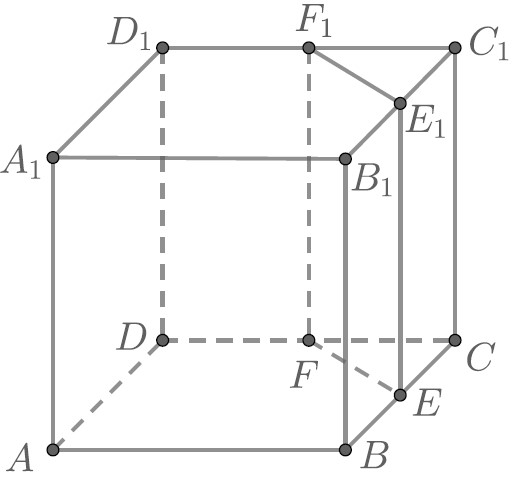
\includegraphics[align=t, width=\linewidth]{\picpath/prob_1_4}
		\end{minipage}
		\item 
		\begin{minipage}[t]{\bodywidth}
			Объем параллелепипеда \(ABCDA_1B_1C_1D_1\) равен \(4,5\). Найдите объем треугольной пирамиды \(AD_1CB_1\).
		\end{minipage}
		\hspace{0.02\linewidth}
		\begin{minipage}[t]{\picwidth}
			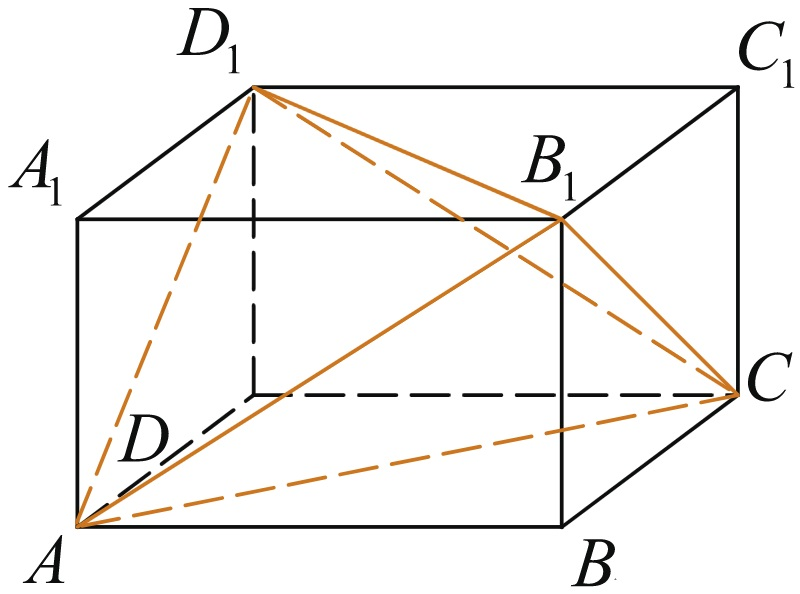
\includegraphics[align=t, width=\linewidth]{\picpath/G112M8L3-1}
		\end{minipage}
		
		\item 
		\begin{minipage}[t]{\bodywidth}
			Объем параллелепипеда \(ABCDA_1B_1C_1D_1\) равен \(9\). Найдите объем треугольной пирамиды \(ABCA_1\).
		\end{minipage}
		\hspace{0.02\linewidth}
		\begin{minipage}[t]{\picwidth}
			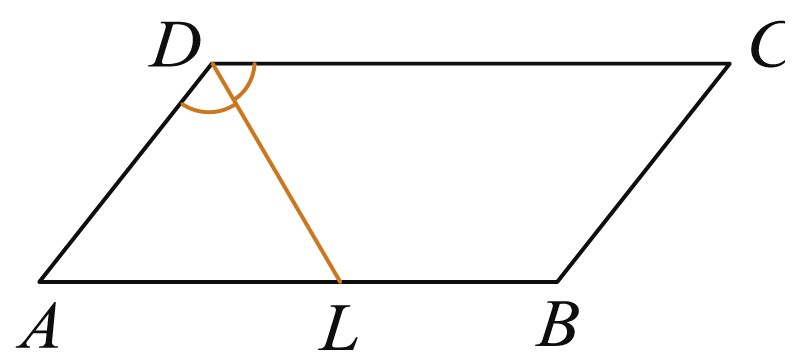
\includegraphics[align=t, width=\linewidth]{\picpath/prob_3_1}
		\end{minipage}
		
		
		%\item Шар вписан в цилиндр. Площадь полной поверхности цилиндра равна \(18\). Найдите площадь поверхности шара.
		\item Прямоугольный параллелепипед описан около цилиндра, радиус основания и высота которого равны \(1\). Найдите объем параллелепипеда.
		\item Цилиндр и конус имеют общие основание и высоту. Найдите объем конуса, если объем цилиндра равен \(150\).
		\item Объем конуса равен \(16\). Через середину высоты параллельно основанию конуса проведено сечение, которое является основанием меньшего конуса с той же вершиной. Найдите объем меньшего конуса.
		\item Во сколько раз увеличится объем конуса, если радиус его основания увеличится в \(1,5\) раза, а высота останется прежней?
		\item Во сколько раз уменьшится объем конуса, если его высота уменьшится в \(3\) раза, а радиус основания останется прежним?
		\item Во сколько раз увеличится площадь боковой поверхности конуса, если его образующая увеличится в \(3\) раза, а радиус основания останется прежним?
		\item Площадь боковой поверхности конуса в два раза больше площади основания. Найдите угол между образующей конуса и плоскостью основания. Ответ дайте в градусах.
		\item Площадь основания конуса равна \(16\pi \), высота --- \(6\). Найдите площадь осевого сечения конуса.
		\item Диаметр основания конуса равен \(6\), а угол при вершине осевого сечения равен \(90\degree \). Вычислите объем конуса, деленный на \(\pi\).
		
		
		
	\end{listofex}
\end{class}
%END_FOLD

%BEGIN_FOLD % ====>>_____ Занятие 4 _____<<====
\begin{class}[number=4]
	\begin{listofex}
		\item Занятие 4
	\end{listofex}
\end{class}
%END_FOLD

%BEGIN_FOLD % ====>>_ Домашняя работа 2 _<<====
\begin{homework}[number=2]
	\begin{listofex}
		\item Высота конуса равна \(4\), а диаметр основания --- \(6\). Найдите образующую конуса.
		\item Площадь основания конуса равна \(16\pi \), высота --- \(6\). Найдите площадь осевого сечения конуса.
		\item Длина окружности основания цилиндра равна \(3\). Площадь боковой поверхности равна \(6\). Найдите высоту цилиндра.
		\item Площадь боковой поверхности цилиндра равна \(2\pi \) , а высота  --- \(1\). Найдите диаметр основания.
		\item Площадь поверхности шара равна \(24\). Найдите площадь большого круга шара.
		\item Во сколько раз уменьшится объем конуса, если его высота уменьшится в \(10\) раз, а радиус основания останется прежним?
		\item Во сколько раз увеличится площадь боковой поверхности конуса, если его образующая увеличится в \(6\) раз, а радиус основания останется прежним?
		\item Площадь поверхности правильной треугольной призмы равна \(6\). Какой станет площадь поверхности призмы, если все её рёбра увеличатся в три раза, а форма останется прежней?
		
		\item Изюм получается в процессе сушки винограда. Сколько килограммов винограда потребуется для получения \(82\) килограммов изюма, если виноград содержит \(90\%\) воды, а изюм содержит \(5\%\) воды?
		\item Смешав \(55\)-процентный и \(97\)-процентный растворы кислоты и добавив \(10\) кг чистой воды, получили \(65\)-процентный раствор кислоты. Если бы вместо \(10\) кг воды добавили \(10\) кг \(50\)-процентного раствора той же кислоты, то получили бы \(75\)-процентный раствор кислоты. Сколько килограммов \(55\)-процентного раствора использовали для получения смеси?
		\item Имеются два сосуда. Первый содержит \(100\) кг, а второй --- \(20\) кг раствора кислоты различной концентрации. Если эти растворы смешать, то получится раствор, содержащий \(67\%\) кислоты. Если же смешать равные массы этих растворов, то получится раствор, содержащий \(77\%\) кислоты. Сколько килограммов кислоты содержится в первом сосуде?
	\end{listofex}
\end{homework}
%END_FOLD

%BEGIN_FOLD % ====>>_____ Занятие 5 _____<<====
\begin{class}[number=5]
	\begin{listofex}
		\item Занятие 5
	\end{listofex}
\end{class}
%END_FOLD

%BEGIN_FOLD % ====>>_____ Занятие 6 _____<<====
\begin{class}[number=6]
	\begin{listofex}
		\item Занятие 6
	\end{listofex}
\end{class}
%END_FOLD

%BEGIN_FOLD % ====>>_ Домашняя работа 3 _<<====
\begin{homework}[number=3]
	\begin{listofex}
		
		%1
		\item В треугольнике \(ABC\): \(AC=BC=27, AH\) --- высота, \(\sin BAC = \dfrac{ 2 }{ 3 }\). Найдите \(BH\).
		%2
		\item Объем куба равен \(24 \sqrt{3}\). Найдите его диагональ.
		%5
		\item Найдите корни уравнения: \( \cos \dfrac{ \pi(x-7) }{ 3 } = 0,5 \).  В ответ запишите наибольший отрицательный корень.
		%6
		\item Вычислить: \(\dfrac{2\sin^221\degree+2\cos^221\degree}{4}\)
		%7
		\item
		\begin{minipage}[t]{\bodywidth}
			На рисунке изображены график функции \(y=f(x)\) и касательная к нему в точке с абсциссой \(x_0\). Найдите значение производной функции \(f(x)\)в точке \(x_0\).
		\end{minipage}
		\hspace{0.02\linewidth}
		\begin{minipage}[t]{\picwidth}
			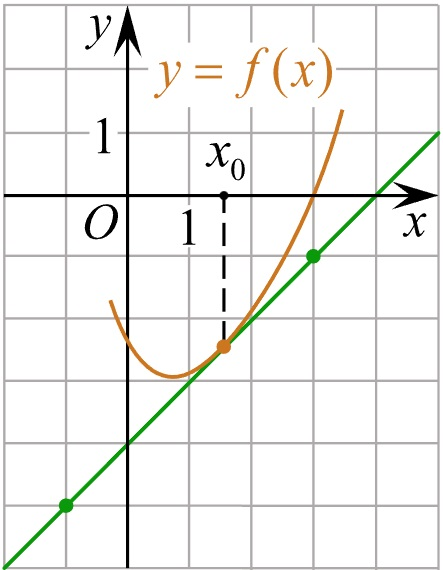
\includegraphics[align=t, width=\linewidth]{\picpath/maksutovM8L4-3}
		\end{minipage}
		%8
		\item После дождя уровень воды в колодце может повыситься. Мальчик измеряет время \(t\) падения небольших камешков в колодец и рассчитывает расстояние до воды по формуле \(h=5t^2\), где \(h\) --- расстояние в метрах, \(t\) --- время падения в секундах. До дождя время падения камешков составляло \(0,6\) с. На сколько должен подняться уровень воды после дождя, чтобы измеряемое время изменилось на \(0,2\) с? Ответ выразите в метрах.
		
		
		%9
		\item В треугольнике \(ABC\): \(CH\) --- высота, \(AD\) --- биссектриса, \(O\) --- точка пересечения прямых \(CH\) и \(AD\), \(\angle BAD = 26 \degree\). Найдите угол \(AOC\). Ответ дайте в градусах.
		%10
		\item
		\begin{minipage}[t]{\bodywidth}
			На рисунке изображён график функции \[ f(x)=a \cos{x}+b \] Найдите \(a\).
		\end{minipage}
		\hspace{0.02\linewidth}
		\begin{minipage}[t]{\picwidth}
			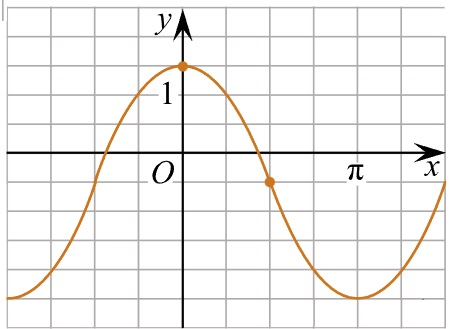
\includegraphics[align=t, width=\linewidth]{\picpath/MECGERM6H3-1}
		\end{minipage}
		%11
		\item Найдите наименьшее значение функции \( y=6 \cos x + \dfrac{ 24 }{ \pi }x+5 \) на отрезке \(\left[ -\dfrac{ 2\pi }{ 3 };0 \right] \).
		
		\item Симметричную монету бросают \(10\) раз. Во сколько раз вероятность события «выпадет ровно \(5\) орлов» больше вероятности события «выпадет ровно \(4\) орла»?
		\item Телефон передаёт \(SMS\)-сообщение. В случае неудачи телефон делает следующую попытку. Вероятность того, что сообщение удастся передать без ошибок в каждой отдельной попытке, равна \(0,4\). Найдите вероятность того, что для передачи сообщения потребуется не больше двух попыток.
		\item При подозрении на наличие некоторого заболевания пациента отправляют на ПЦР-тест. Если заболевание действительно есть, то тест подтверждает его в \(86\%\) случаев. Если заболевания нет, то тест выявляет отсутствие заболевания в среднем в \(94\%\) случаев. Известно, что в среднем тест оказывается положительным у \(10\%\) пациентов, направленных на тестирование.
		При обследовании некоторого пациента врач направил его на ПЦР-тест, который оказался положительным. Какова вероятность того, что пациент действительно имеет это заболевание?
		\item В ящике четыре красных и два синих фломастера. Фломастеры вытаскивают по очереди в случайном порядке. Какова вероятность того, что первый раз синий фломастер появится третьим по счету?
		\item При выпечке хлеба производится контрольное взвешивание свежей буханки. Известно, что вероятность того, что масса окажется меньше, чем \(810\) г, равна \(0,97\). Вероятность того, что масса окажется больше, чем \(790\) г, равна \(0,91\). Найдите вероятность того, что масса буханки больше, чем \(790\) г, но меньше, чем \(810\) г.
		\item %484557
		\begin{tasks}(1)
			\task Решите уравнение \( (2\sin x+\sqrt{3}) \cdot \sqrt{\cos x}=0 \)
			\task Найдите все корни этого уравнения, принадлежащие отрезку: \( \left[ \dfrac{3\pi}{2}; \dfrac{7\pi}{2} \right] \)
		\end{tasks}
		\item %505102
		\begin{tasks}(1)
			\task Решите уравнение \( 9^{\sin{x}}+9^{-\sin x}=\dfrac{10}{3} \)
			\task Найдите все корни этого уравнения, принадлежащие отрезку: \( \left[ -\dfrac{7\pi}{2}; -2\pi \right]  \)
		\end{tasks}
		\newpage
		\item %505236
		\begin{tasks}(1)
			\task Решите уравнение \( \left( \dfrac{2}{5} \right)^{\cos x}+ \left( \dfrac{5}{2} \right)^{\cos x}=2 \)
			\task Найдите все корни этого уравнения, принадлежащие отрезку: \( \left[ -3\pi;-\dfrac{3\pi}{2} \right]  \)
		\end{tasks}
	\end{listofex}
\end{homework}
%END_FOLD

%BEGIN_FOLD % ====>>_____ Занятие 7 _____<<====
\begin{class}[number=7]
	\begin{listofex}
		\item В банк был положен вклад под \(10\%\) годовых. Через год, после начисления процентов, вкладчик снял со счета \(2000\) рублей, а еще через год (опять после начисления процентов) снова внес \(2000\) рублей. Вследствие этих действий через три года со времени открытия вклада вкладчик получил сумму меньше запланированной (если бы не было промежуточных операций со вкладом). На сколько рублей меньше запланированной суммы он получил?
		\item Василий кладет в банк \(1 000 000\) рублей под \(10\%\) годовых на \(4\) года (проценты начисляются один раз после истечения года) с правом докладывать три раза (в конце каждого года после начисления процентов) на счет фиксированную сумму \(133 000\) рублей. Какая максимальная сумма может быть на счете у Василия через \(4\) года?
		\item В банк помещена сумма \(3900\) тысяч рублей под \(50\%\) годовых. В конце каждого из первых четырех лет хранения после начисления процентов вкладчик дополнительно вносил на счет одну и ту же фиксированную сумму. К концу пятого года после начисления процентов оказалось, что размер вклада увеличился по сравнению с первоначальным на \(725\%\). Какую сумму вкладчик ежегодно добавлял к вкладу?
		\item Антон взял кредит в банке на срок \(6\) месяцев. В конце каждого месяца общая сумма оставшегося долга увеличивается на одно и то же число процентов (месячную процентную ставку), а затем уменьшается на сумму, уплаченную Антоном. Суммы, выплачиваемые в конце каждого месяца, подбираются так, чтобы в результате сумма долга каждый месяц уменьшалась равномерно, то есть на одну и ту же величину. Общая сумма выплат превысила сумму кредита на \(63\%\). Найдите месячную процентную ставку.
		\item Жанна взяла в банке в кредит \(1,2\) млн рублей на срок \(24\) месяца. По договору Жанна должна вносить в банк часть денег в конце каждого месяца. Каждый месяц общая сумма долга возрастает на \(2\%\), а затем уменьшается на сумму, уплаченную Жанной банку в конце месяца. Суммы, выплачиваемые Жанной, подбираются так, чтобы сумма долга уменьшалась равномерно, то есть на одну и ту же величину каждый месяц. Какую сумму Жанна выплатит банку в течение первого года кредитования?
		\newpage
		\item В июле планируется взять кредит в банке на некоторую сумму. Условия его возврата таковы:\\
		--- каждый январь долг возрастает на \(31\%\) по сравнению с концом предыдущего года;\\
		--- с февраля по июнь каждого года необходимо выплатить часть долга, равную \(69 690 821\) рубль.\\
		Сколько рублей было взято в банке, если известно, что он был полностью погашен тремя равными платежами (то есть за три года)?
	\end{listofex}
\end{class}
%END_FOLD

%BEGIN_FOLD % ====>>_ ДЗ 4 _<<====
\begin{homework}[number=4]
	\begin{listofex}
		\item \(31\) декабря \(2014\) года Савелий взял в банке \(7 378 000\) рублей в кредит под \(12,5\%\) годовых. Схема выплаты кредита следующая: \(31\) декабря каждого следующего года банк начисляет проценты на оставшуюся сумму долга (то есть увеличивает долг на \(12,5\%\)), затем Савелий Переводит в банк платёж. Весь долг Савелий выплатил за \(3\) равных платежа. На сколько рублей меньше он бы отдал банку, если бы смог выплатить долг за \(2\) равных платежа?
		\item Ольга хочет взять в кредит \(100 000\) рублей под \(10\%\) годовых. Погашение кредита происходит раз в год равными суммами (кроме, может быть, последней) после начисления процентов. На какое минимальное количество лет Ольга может взять кредит, чтобы ежегодные выплаты были не более \(24\) тысяч рублей?
		\item В июле \(2016\) года планируется взять кредит в размере \(6,6\) млн. руб. Условия возврата таковы: \\
		--- каждый январь долг возрастает на \(r\%\) по сравнению с концом предыдущего года. \\
		--- с февраля по июнь необходимо выплатить часть долга. \\
		--- в июле \(2017, 2018\) и \(2019\) годов долг остается равным \(6,6\) млн. руб. \\
		--- суммы выплат \(2020\) и \(2021\) годов равны. \\
		Найдите \(r\), если в \(2021\) году долг будет выплачен полностью и общие выплаты составят \(12,6\) млн. рублей.
		\item \(15\)-го января планируется взять кредит в банке на шесть месяцев в размере \(1\) млн рублей. Условия его возврата таковы: \\
		--- \(1\)-го числа каждого месяца долг увеличивается на \(r\) процентов по сравнению с концом предыдущего месяца, где \(r\) --- целое число; \\
		--- со \(2\)-го по \(14\)-е число каждого месяца необходимо выплатить часть долга; \\
		--- \(15\)-го числа каждого месяца долг должен составлять некоторую сумму в соответствии со следующей таблицей. \\
		\begin{table}[h]
			\begin{tabular}{|l|
					>{\columncolor[HTML]{FFFFFF}}c |
					>{\columncolor[HTML]{FFFFFF}}c |
					>{\columncolor[HTML]{FFFFFF}}c |
					>{\columncolor[HTML]{FFFFFF}}c |
					>{\columncolor[HTML]{FFFFFF}}c |
					>{\columncolor[HTML]{FFFFFF}}c |
					>{\columncolor[HTML]{FFFFFF}}c |}
				\hline
				Дата                & 15.01 & 15.02 & 15.03 & 15.04 & 15.05 & 15.06 & 15.07 \\ \hline
				Долг (в млн рублей) & 1     & 0,6   & 0,4   & 0,3   & 0,2   & 0,1   & 0     \\ \hline
			\end{tabular}
		\end{table}
		%\begin{minipage}[t]{\linewidth}
		%	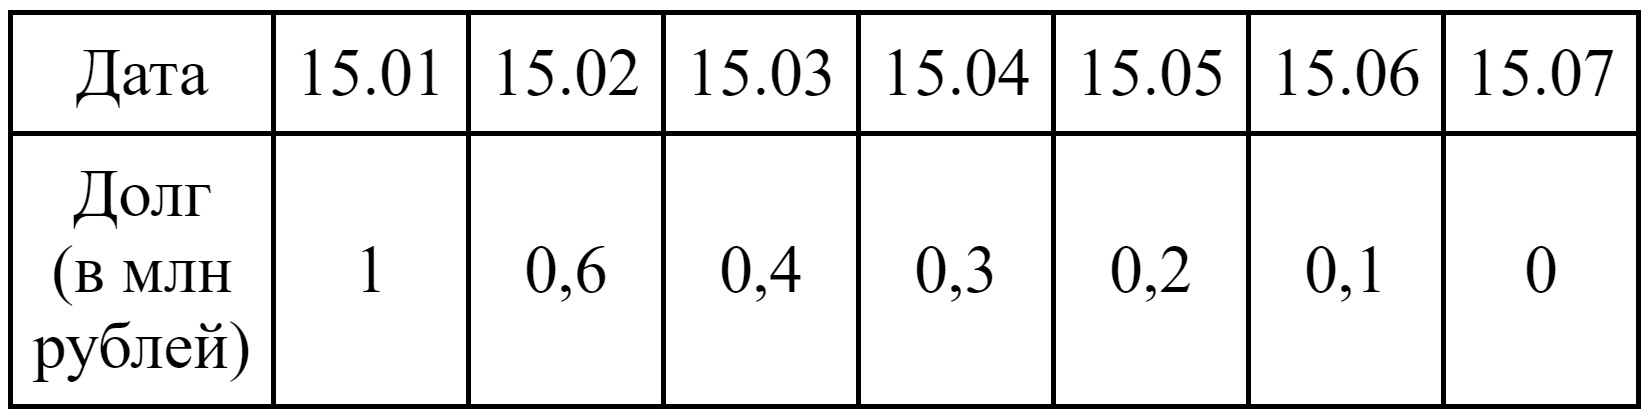
\includegraphics[align=t, width=\linewidth]{\picpath/G112M9H4-1}
		%\end{minipage}
		\\
		Найдите наибольшее значение \(r\), при котором общая сумма выплат будет меньше \(1,2\) млн рублей.
		
		\item \(15\)-го января планируется взять кредит в банке на сумму \(2,4\) млн рублей на \(24\) месяца. Условия его возврата таковы: \\
		--- \(1\)-го числа каждого месяца долг возрастает на \(3\%\) по сравнению с концом предыдущего месяца; \\
		--- со \(2\)-го по \(14\)-е число каждого месяца необходимо выплатить часть долга; \\
		--- \(15\)-го числа каждого месяца долг должен быть на одну и ту же величину меньше долга на \(15\)-е число предыдущего месяца. \\
		Какую сумму нужно выплатить банку в первые \(12\) месяцев?
	\end{listofex}
\end{homework}
%END_FOLD

%BEGIN_FOLD % ====>>_ Консультация Борисов _<<====
\begin{consultation}
	\begin{listofex}
		\item Найдите площадь треугольника, две стороны которого равны \(8\) и \(12\), а угол между ними равен \(30 \degree\).
		\item Большее основание равнобедренной трапеции равно \(34\). Боковая сторона равна \(14\). Синус острого угла равен \( \dfrac{ 2\sqrt{10}}{ 7 } \). Найдите меньшее основание.
		%\item Основания равнобедренной трапеции равны \(7\) и \(51\). Тангенс острого угла равен \( \dfrac{ 5 }{ 11 } \).  Найдите высоту трапеции.
		%\item Большее основание равнобедренной трапеции равно \(34\). Боковая сторона равна \(14\). Синус острого угла равен \( \dfrac{ 2\sqrt{10}}{ 7 } \). Найдите меньшее основание.
		\item Основания равнобедренной трапеции равны \(7\) и \(51\). Тангенс острого угла равен \( \dfrac{ 5 }{ 11 } \).  Найдите высоту трапеции.
		\item В параллелограмме \( ABCD: \quad AB  =  3, AD  =  21, \sin A = \dfrac{ 6 }{ 7 } \). Найдите большую высоту параллелограмма.
		\item Найдите площадь ромба, если его высота равна \(2\), а острый угол \(30\degree \).
		\item Периметр треугольника равен \(12\), а радиус вписанной окружности равен \(1\). Найдите площадь этого треугольника.
		\item Найдите радиус окружности, вписанной в правильный треугольник, высота которого равна \(6\).
		\item Сторона правильного треугольника равна \(\sqrt{3}\). Найдите радиус окружности, описанной около этого треугольника.
		\item Найдите сторону правильного шестиугольника, описанного около окружности, радиус которой равен \(\sqrt{3}\).
		\item Чему равна сторона правильного шестиугольника, вписанного в окружность, радиус которой равен \(6\)?
		\item Даны два шара. Радиус первого шара в \(2\) раза больше радиуса второго. Во сколько раз площадь поверхности первого шара больше площади поверхности второго?
		\item Шар вписан в цилиндр. Площадь полной поверхности цилиндра равна \(18\). Найдите площадь поверхности шара.
		\item Прямоугольный параллелепипед описан около цилиндра, радиус основания и высота которого равны \(1\). Найдите объем параллелепипеда.
		\item Объем первого цилиндра равен \(12\) м\(^3\). У второго цилиндра высота в три раза больше, а радиус основания --- в два раза меньше, чем у первого. Найдите объем второго цилиндра. Ответ дайте в кубических метрах.
		\item В цилиндрический сосуд налили \(2000\) см\(^3\) воды. Уровень воды при этом достигает высоты \(12\) см. В жидкость полностью погрузили деталь. При этом уровень жидкости в сосуде поднялся на \(9\) см. Чему равен объем детали? Ответ выразите в см\(^3\).
		\item Объем конуса равен \(16\). Через середину высоты параллельно основанию конуса проведено сечение, которое является основанием меньшего конуса с той же вершиной. Найдите объем меньшего конуса.
		\item В сосуд, имеющий форму правильной треугольной призмы, налили \(2300\) см\(^3\) воды и погрузили в воду деталь. При этом уровень воды поднялся с отметки \(25\) см до отметки \(27\) см. Найдите объем детали. Ответ выразите в см\(^3\).
	\end{listofex}
\end{consultation}

%BEGIN_FOLD % ====>>_ Консультация Борисов _<<====
\begin{consultation}
	\begin{listofex}
		%???chelnokovam5
		\item Вычислить: 
		\begin{tasks}(2)
			\task \( \dfrac{5\cos29\degree}{\sin61\degree} \)
			\task \( -4\sqrt{3}\cos(-750\degree) \)
			\task \( \dfrac{4\cos146\degree}{\cos34\degree} \)
			\task \( 7\tg13\degree\cdot\tg77\degree \)
			\task \( \dfrac{12}{\sin^227\degree+\cos^2207\degree} \)
			\task \( \dfrac{5\sin98\degree}{\sin49\degree\cdot\sin41\degree} \)
			\task \( -50\tg9\degree\cdot\tg81\degree+31 \)
		\end{tasks}
		\item Вычислить: %114m3
		\begin{tasks}(2)
			\task \( \dfrac{-13\sin126\degree}{\sin54\degree} \)
			\task \( \cos^2(-46\degree)+\sin^2(-46\degree) \)
			\task \( \sin^223\degree+9+\cos^223 \)
			\task \( \dfrac{2\sin^221\degree+2\cos^221\degree}{4} \)
		\end{tasks}
		%n5 cos1
		\item Найдите корни уравнения: \( \cos \dfrac{ \pi(x-7) }{ 3 } = 0,5 \).  В ответ запишите наибольший отрицательный корень.
		%n5 cos3
		\item Найдите корни уравнения: \( \cos \dfrac{ \pi(2x+9) }{ 3 } = \dfrac{ \sqrt{2} }{ 2 } \).  В ответ запишите наибольший отрицательный корень.
		%n5 sin1
		\item Найдите корни уравнения: \( \sin \dfrac{ \pi x }{ 3 } = 0,5 \).  В ответ запишите наименьший положительный корень.
		%n5 tg1
		\item Найдите корни уравнения: \( \tg \dfrac{ \pi x }{ 4 } = -1 \).  В ответ запишите наибольший отрицательный корень.
		%n5 tg2
		\item Найдите корни уравнения: \( \tg \dfrac{ \pi (x+2) }{ 3 } = -\sqrt{3} \).  В ответ запишите наибольший отрицательный корень.
		\item Найдите: %101L1
		\begin{tasks}
			\task \( 5\sin\alpha \), если \( \cos\alpha=\dfrac{2\sqrt{6}}{5} \) и \( \alpha\in\left( \dfrac{3\pi}{2}; 2\pi \right) \);
			\task \( 3\cos\alpha \), если \( \sin\alpha=-\dfrac{2\sqrt{2}}{3} \) и \( \alpha\in\left( \dfrac{3\pi}{2}; 2\pi \right) \);
			\task \( 24\cos\alpha \), если \( \sin\alpha=-0,2 \);
			\task \( \sin\left( \dfrac{7\pi}{2}-\alpha \right) \), если \( \sin\alpha=0,8 \) и \( \alpha\in\left( \dfrac{\pi}{2}; \pi \right) \).
		\end{tasks}
		\item При нормальном падении света с длиной волны \( \lambda=400 \) нм на дифракционную решeтку с периодом \(d\) нм наблюдают серию дифракционных максимумов. При этом угол \(\varphi\)  (отсчитываемый от перпендикуляра к решeтке), под которым наблюдается максимум, и номер максимума \(k\) связаны соотношением \(d \sin \varphi= k\lambda\). Под каким минимальным углом \(\varphi\) (в градусах) можно наблюдать второй максимум на решeтке с периодом, не превосходящим \(1600\) нм?
		%priklad trigon 2
		\item Два тела массой \(m=2\) кг каждое, движутся с одинаковой скоростью  \(v =10\) м/с под углом \(2\alpha\) друг к другу. Энергия (в джоулях), выделяющаяся при их абсолютно неупругом соударении определяется выражением \(Q= m v^2 \sin^2 \alpha \). Под каким наименьшим углом \(2\alpha\) (в градусах) должны двигаться тела, чтобы в результате соударения выделилось не менее \(50\) джоулей?
	\end{listofex}
\end{consultation}

%BEGIN_FOLD % ====>>_ class 9 _<<====
\begin{class}[number=9]
	\begin{listofex}
		%\item Известно, что вклад, находящийся в банке с начала года, возрастает к концу года на определенный процент, свой для каждого банка. В начале года Степан положил \(60\%\) некоторой суммы денег в первый банк, а оставшуюся часть суммы во второй банк. К концу года сумма этих вкладов стала равна \(590 000\) руб., а к концу следующего года \(701 000\) руб. Если бы Степан первоначально положил \(60\%\) своей суммы во второй банк, а оставшуюся часть в первый, то по истечении одного года сумма вкладов стала бы равной \(610 000\) руб. Какова была бы сумма вкладов в этом случае к концу второго года?
		%\item По бизнес-плану предполагается изначально вложить в четырёхлетний проект \(10\) млн рублей. По итогам каждого года планируется прирост вложенных средств на \(15\%\) по сравнению с началом года. Начисленные проценты остаются вложенными в проект. Кроме этого, сразу после начислений процентов нужны дополнительные вложения: по целому числу \(n\) млн рублей в первый и второй годы, а также по целому числу \(m\) млн рублей в третий и четвёртый годы.
		%Найдите наименьшие значения \(n\) и \(m\), при которых первоначальные вложения за два года как минимум удвоятся, а за четыре года как минимум утроятся.
		\item Сергей взял кредит в банке на срок \(9\) месяцев. В конце каждого месяца общая сумма оставшегося долга увеличивается на \(12\%\), а затем уменьшается на сумму, уплаченную Сергеем. Суммы, выплачиваемые в конце каждого месяца, подбираются так, чтобы в результате сумма долга каждый месяц уменьшалась равномерно, то есть на одну и ту же величину. Сколько процентов от суммы кредита составила сумма, уплаченная Сергеем банку сверх кредита?
		\item \(1\) января \(2015\) года Павел Витальевич взял в банке \(1\) млн рублей в кредит. Схема выплаты кредита следующая: \(1\) числа каждого следующего месяца банк начисляет \(1\) процент на оставшуюся сумму долга (то есть увеличивает долг на \(1\%\)), затем Павел Витальевич переводит в банк платёж. На какое минимальное количество месяцев Павел Витальевич может взять кредит, чтобы ежемесячные выплаты были не более \(125\) тыс. рублей?
		\item \(15\)-го января был выдан полугодовой кредит на развитие бизнеса. В таблице представлен график его погашения. \\
		В конце каждого месяца, начиная с января, текущий долг увеличивался на \(5\%\), а выплаты по погашению кредита происходили в первой половине каждого месяца, начиная с февраля. На сколько процентов общая сумма выплат при таких условиях больше суммы самого кредита?
		\begin{table}[h]
			\begin{tabular}{|
					>{\columncolor[HTML]{DEDEDE}}c |
					>{\columncolor[HTML]{FFFFFF}}c |
					>{\columncolor[HTML]{FFFFFF}}c |
					>{\columncolor[HTML]{FFFFFF}}c |
					>{\columncolor[HTML]{FFFFFF}}c |
					>{\columncolor[HTML]{FFFFFF}}c |
					>{\columncolor[HTML]{FFFFFF}}c |
					>{\columncolor[HTML]{FFFFFF}}c |}
				\hline
				\textbf{Дата}                          & 15.01 & 15.02 & 15.03 & 15.04 & 15.05 & 15.06 & 15.07 \\ \hline
				\textbf{Долг (в процентах от кредита)} & 100\% & 90\%  & 80\%  & 70\%  & 60\%  & 50\%  & 0\%   \\ \hline
			\end{tabular}
		\end{table}
	\end{listofex}
\end{class}